\chapter{Results and analysis}

We performed classification with 4 different classifiers on 4 different datasets. In each dataset-classifier we measured each classification accuracy when applying 4 different feature selection (FS) methods. The aim is to investigate the impact of feature selection, and the interaction between different classifiers and FS-methods. To build a basis for comparisons classification accuracy was measured without FS too.

\section{Variation among factors of experiments}
\label{Variation_among_factors}

Before analyzing the results we must consider potential interaction between the different factors involved in the experiment, these are:

\begin{enumerate}
  \item Datasets
  \item Machine Learning classifiers
  \item Feature selection methods
\end{enumerate}

As we have four of each the there are 64 different combinations of these factors. We are interested of two interactions in particular:

\begin{itemize}
  \item \textbf{1 * 3} Because this interaction renders...
  \item \textbf{2 * 3} Because this interaction renders...
\end{itemize}

To study these interactions we performed anova... See below...

\subsection{FS-methods is dataset dependent}

Comparing the accuracy of each method with respect to the datasets shows a positive correlation, as visualised in plot \ref{fig:comp_acc_datasets}. The correlation indicates datasets with a larger amount of features benefit more from feature selection than datasets with smaller amount of features.

% ANOVA plots
\begin{figure*}[ht]
  \centering
    \begin{subfigure}[b]{0.475\textwidth}
        \centering
        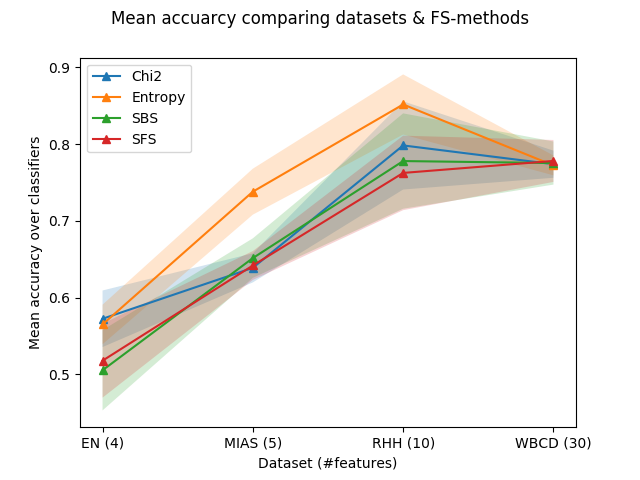
\includegraphics[width=\textwidth]{../plots_with_std_fill/comp_acc_datasets.png}
        \caption[]%
        {{\small Datasets and accuracy displays evident correlation independently of applied FS method.}}
        \label{fig:comp_acc_datasets}
    \end{subfigure}
  \hfill
    \begin{subfigure}[b]{0.475\textwidth}
        \centering
        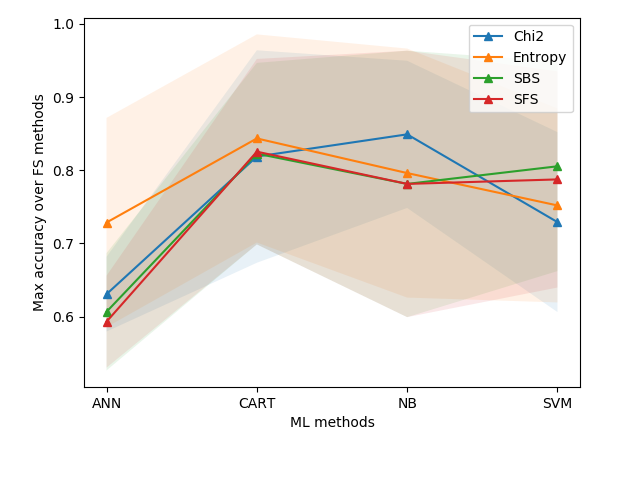
\includegraphics[width=\textwidth]{../plots_with_std_fill/comp_classif_datasets.png}
        \caption[]%
        {{\small Some correlation between different classifiers and FS-methods is evident.}}
        \label{fig:comp_classif_datasets}
    \end{subfigure}
  \caption[]
  {\small Good caption goes here.}
  \label{fig:anova_plots}
\end{figure*}


ANOVA shows a statistical significance in the correlation due to the found values of the test, table \ref{table:anova_values_data}. The significance is evident due to the very small value $P(>F)$, probability of not rejecting the null hypothesis. Thus we can confidently reject the null hypothesis which is datasets are significantly the same in respect to FS-methods.

% ANOVA computations, dataset-fs
\begin{table}[ht]
  \begin{center}
  \begin{tabular}{l|r|r|r|r|r|r|}
  \cline{2-7}
  & $RSS$ & $df$ & $F$ & $P(>F)$ & $\eta^2$ & $\omega^2$ \\ \cline{1-7}
  \multicolumn{1}{ |l| }{\textbf{Dataset}}
  & 0.7383 &  3.0 & 15.939 & 2.5241e-07 & 0.4757 & 0.4415 \\
  \cline{1-7}
  \multicolumn{1}{ |l| }{\textbf{Method}}
  & 0.0099 &  3.0 & 0.2137 & 8.8645e-01 & 0.0064 & -0.0232 \\
  \cline{1-7}
  \multicolumn{1}{ |l| }{\textbf{Dataset:Method}}
  & 0.0627 &  9.0 & 0.4514 & 8.9938e-01 & 0.0404 & -0.0486 \\
  \cline{1-7}
  \multicolumn{1}{ |l| }{\textbf{Residual}}
  & 0.7412 &  48.0 \\ \cline{1-3}
  \end{tabular}
  \caption{ANOVA values of accuracy in relation to dataset, method and the interaction of datasets and methods.}
  \label{table:anova_values_data}
  \end{center}
\end{table}


\subsection{FS-methods are classifier dependent}

We regarded datasets as an independent variable and compared classification accuracy between different classifiers and FS-methods. The plot in \ref{fig:comp_classif_datasets} visualizes the correlation between different classifiers and FS-methods...

Performing 2-way anova showed the interaction between classifier-fs combinations are significantly different with a p-value of X. The values are presented in table \ref{table:anova_values_classif}.

This means... It is particularly interesting because wrapper methods uses classifiers as a black box and should to our understanding be classifier independent.

\begin{table}[ht]
  \begin{center}
  \begin{tabular}{l|r|r|r|r|r|r|}
  \cline{2-7}
  & $RSS$ & $df$ & $F$ & $P(>F)$ & $\eta^2$ & $\omega^2$ \\ \cline{1-7}
  \multicolumn{1}{ |l| }{\textbf{Classifier}}
  & 0.3336 &  3.0 & 16.491 & 1.6860e-07 & 0.2149 & 0.2010 \\
  \cline{1-7}
  \multicolumn{1}{ |l| }{\textbf{Method}}
  & 0.7383 &  3.0 & 36.495 & 1.9503e-12 & 0.4757 & 0.4607 \\
  \cline{1-7}
  \multicolumn{1}{ |l| }{\textbf{Classifier*Method}}
  & 0.1565 &  9.0 & 2.5783 & 1.6490e-02 & 0.1008 & 0.0614 \\
  \cline{1-7}
  \multicolumn{1}{ |l| }{\textbf{Residual}}
  & 0.3237 &  48.0 \\ \cline{1-3}
  \end{tabular}
  \caption{Set caption.}
  \label{table:anova_values_classif}
  \end{center}
\end{table}



\section{Classification improvements}

After performing classification with and without available FS-methods we compared the classification accuracies in tables \ref{table:ANN}, \ref{table:NB}, \ref{table:SVM} and \ref{table:CART}.

The tables showed that predominantly classification accuracy is improved for all classifiers tested in our scope by use of \textit{some} feature selection method. Results presented in tables corresponding to ANN \ref{table:ANN}, NB \ref{table:NB} and SVM \ref{table:SVM} entails comparing the best performing FS-method to a full dataset consistently results in equal or improved accuracy. Only in DT \ref{table:CART} one dataset exists that performed better without feature selection.

However, majority of the classifiers had some FS-method that achieved lower accuracy compared to full dataset. In 11 of 16 instances at least one FS-method performed worse. This is in line with our findings that FS-method is both dataset and classifier dependent. Further it suggests one have to select the combination of classifier and FS-method carefully.

% --- Tables ---
\begin{table}[h]
  \begin{tabular}{|l|l|l|l|l|l}
\cline{1-5}
        \textbf{ANN} & MIAS              & EN                & RHH               & WBCD      &         \\
\cline{1-5}
Chi2    & 0.58 & 0.59 & 0.64 & 0.71 \\
Entropy & 0.56 & \textbf{0.84} & \textbf{0.90} & 0.62 \\
SBS     & 0.54 & 0.55 & 0.59 & \textbf{0.74} \\
SFS     & \textbf{0.59} & 0.51 & 0.59 & 0.68 \\
Full    & 0.57 & 0.68 & 0.60 & 0.53 \\
\cline{1-5}
Gain    & 0.04 & 0.24 & 0.51 & 0.41 & 1.2 \\
\cline{1-5}
\end{tabular}

  \caption[]%
  {{\small Classification accuracy achieved by ANN was improved on all datasets by the use of some feature selection method.}}
  \label{table:ANN}
\end{table}

\begin{table}[h]
  \begin{tabular}{|l|l|l|l|l|l}
\cline{1-5}
        \textbf{CART} & MIAS              & EN                & RHH               & WBCD      &         \\
\cline{1-5}
Chi2    & 0.70           & 0.69           & 0.90           & \textbf{0.97}  &         \\
Entropy & 0.53           & \textbf{0.83}  & 0.91           & 0.96           &         \\
SBS     & 0.63           & 0.67           & 0.91           & 0.95           &         \\
SFS     & 0.67           & 0.67           & \textbf{0.92}  & \textbf{0.97}  &         \\
Full    & \textbf{0.77}  & 0.69           & 0.90           & 0.94           &         \\
\cline{1-5}
\cline{1-5}
Gain    & -0.09           & 0.21           & 0.03           & 0.03           & 0.18 \\
\cline{1-5}
\end{tabular}
 \\
  \caption[]%
  {{\small All datasets except MIAS benefited from feature selection using CART Decision Tree classifier.}}
  \label{table:CART}
\end{table}

\begin{table}[h]
  \begin{tabular}{|l|l|l|l|l|l}
\cline{1-5}
        & MIAS              & EN                & RHH               & WBCD      &         \\
\cline{1-5}
Chi2    & \textbf{0.77}  & \textbf{0.74}  & \textbf{0.94}  & 0.96           &         \\
Entropy & \textbf{0.77}  & 0.55           & 0.91           & 0.97           &         \\
SBS     & 0.43           & 0.71           & 0.91           & \textbf{0.97}  &         \\
SFS     & 0.43           & 0.71           & 0.91           & \textbf{0.97}  &         \\
Full    & \textbf{0.77}  & 0.66           & \textbf{0.94}  & 0.96           &         \\
\cline{1-5}
\cline{1-5}
Gain    & 0                 & 0.12           & 0                 & 0.01           & 0.14 \\
\cline{1-5}
\end{tabular}
 \\
  \caption[]%
  {{\small Naive Bayes sees improvement or equivalent accuracy by feature selection on every dataset.}}
  \label{table:NB}
\end{table}

\begin{table}[h]
  \begin{tabular}{|l|l|l|l|l|l}
\cline{1-5}
        \textbf{SVM} & MIAS              & EN                & RHH               & WBCD      &         \\
\cline{1-5}
Chi2    & \textbf{0.57}  & 0.73           & 0.90           & 0.63           &         \\
Entropy & 0.33           & \textbf{0.83}  & \textbf{0.91}  & 0.63           &         \\
SBS     & 0.53           & 0.68           & 0.88           & \textbf{0.93}  &         \\
SFS     & 0.53           & 0.68           & 0.88           & \textbf{0.93}  &         \\
Full    & \textbf{0.57}  & 0.73           & 0.90           & 0.61           &         \\
\cline{1-5}
\cline{1-5}
Gain    & 0                 & 0.14           & 0.02           & 0.51           & 0.68 \\
\cline{1-5}
\end{tabular}
 \\
  \caption[]%
  {{\small Classification accuracy achieved by SVM was improved or equivalent on every dataset with use of feature selection.}}
  \label{table:SVM}
\end{table}
% ---/Tables ---


\subsection{Differences among classifiers}

We found there is a large variance between results depending on which dataset, classifier and FS-method that is applied. These findings was addressed in section \ref{Variation_among_factors}. Here we further analyze these differences.

Each plot \ref{fig:plots_chi2}, \ref{fig:plots_entropy}, \ref{fig:plots_sbs} and \ref{fig:plots_sfs} represents one feature selection method. The subplots, like \ref{fig:RHH_chi2} visualises the classification accuracy on one dataset in respect to number of features.

\begin{table}[hp]
  \begin{tabular}{|l|l|l|l|}
\hline
Ranking  & Classifier                & Accumulated gain  & Average gain\\
\hline
1        & Artificial Neural Network & 1.34   & 34\%        \\
2        & Support Vector Machine    & 0.68  & 17\%       \\
3        & Decision Tree             & 0.18   & 5\%         \\
4        & Naïve Bayes               & 0.14   & 4\%         \\
\hline
\end{tabular}

  \caption[]%
  {{\small Ranking of which classifiers gained most accuracy when comparing feature selection to full dataset.}}
  \label{table:gain_comparison}
\end{table}

\subsubsection{Artificial Neural Network}

Looking at the table \ref{table:gain_comparison} the accumulated gain was 1.34 which was the highest among all classifiers. However, ANN consistently performs the worst of all classifiers in terms of accuracy. The ANN also provides the least consistent results with strong fluctuations in the results and wide standard deviation margins. Such fluctuations may suggest issues regarding convergence. These characteristics are evident in plot \ref{fig:WBCD_chi2}.

\begin{figure*}[htp]
  \centering
  \begin{subfigure}[b]{0.475\textwidth}
      \centering
      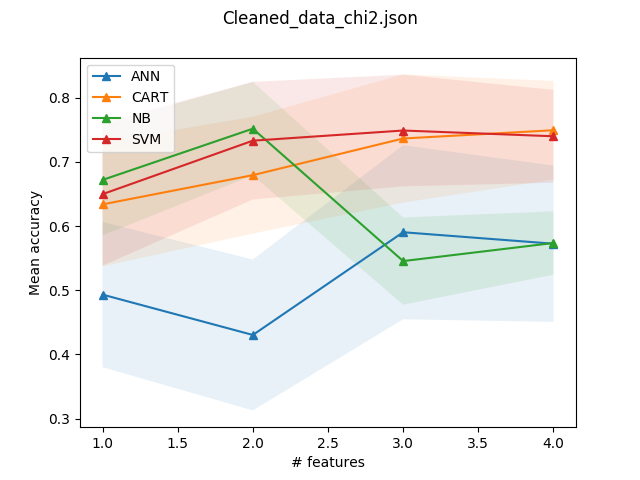
\includegraphics[width=\textwidth]{../plots_with_std_fill/Cleaned_data_chi2_combined.png}
      \caption[]%
      {{\small}}
      \label{fig:EN_chi2}
  \end{subfigure}
  \hfill
  \begin{subfigure}[b]{0.475\textwidth}
      \centering
      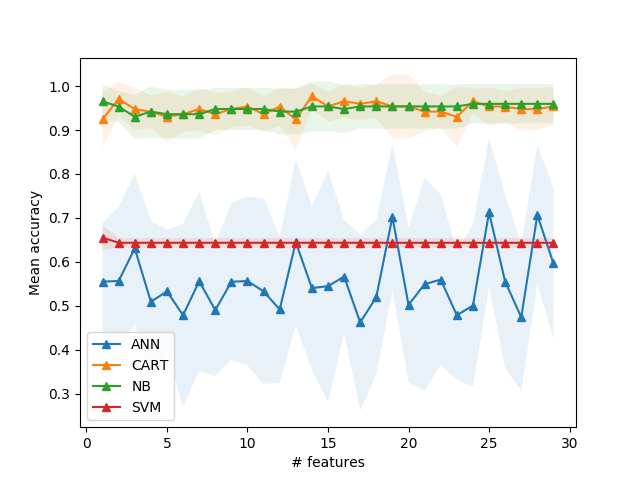
\includegraphics[width=\textwidth]{../plots_with_std_fill/data_FNA_chi2_combined.png}
      \caption[]%
      {{\small}}
      \label{fig:WBCD_chi2}
  \end{subfigure}
  \vskip\baselineskip
  \begin{subfigure}[b]{0.475\textwidth}
      \centering
      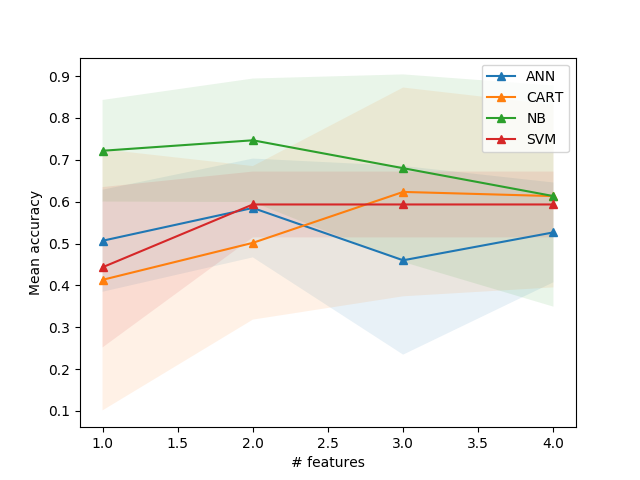
\includegraphics[width=\textwidth]{../plots_with_std_fill/Data_mias_chi2_combined.png}
      \caption[]%
      {{\small}}
      \label{fig:MIAS_chi2}
  \end{subfigure}
  \quad
  \begin{subfigure}[b]{0.475\textwidth}
      \centering
      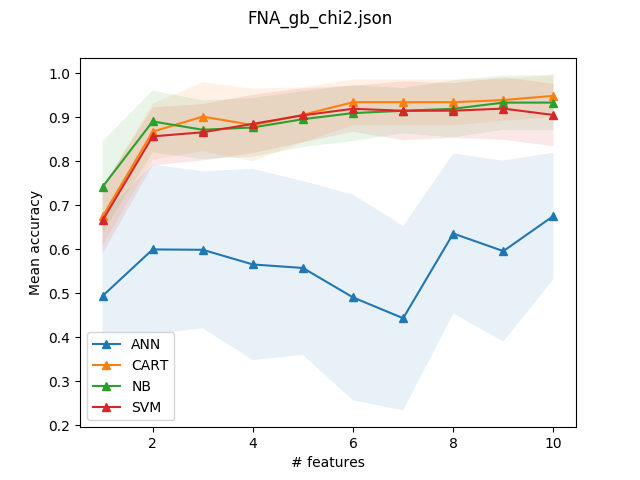
\includegraphics[width=\textwidth]{../plots_with_std_fill/FNA_gb_chi2_combined.png}
      \caption[]%
      {{\small}}
      \label{fig:RHH_chi2}
  \end{subfigure}
  \caption[]
  {\small a: Dataset EN using Chi2, b: Dataset WBCD using Chi2, c:  Dataset MIAS using Chi2, d: Dataset RHH using Chi2.  Combined plots of all datasets comparing each classifier when using chi2 for feature selection.}
  \label{fig:plots_chi2}
\end{figure*}


\subsubsection{Support Vector Machine}

The SVM behaves very differently in respect to each dataset. Improvements are seen with a larger subset of attributes in the EN and MIAS dataset as seen in \ref{fig:EN_chi2} and \ref{fig:MIAS_sfs}. A negative trend on accuracy is observed on the WBCD datasets which might indicate an issue with dimensionality. In \ref{fig:RHH_sbs} an improved accuracy is evident with maximal accuracy achieved on a subset suggesting a positive effect of feature selection.

\begin{figure*}[htp]
  \centering
  \begin{subfigure}[b]{0.475\textwidth}
      \centering
      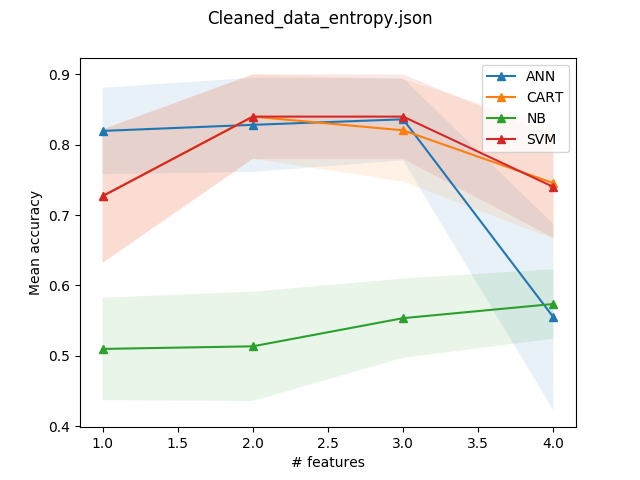
\includegraphics[width=\textwidth]{../plots_with_std_fill/Cleaned_data_entropy_combined.png}
      \caption[Network2]%
      {{\small }}
      \label{fig:EN_entropy}
  \end{subfigure}
  \hfill
  \begin{subfigure}[b]{0.475\textwidth}
      \centering
      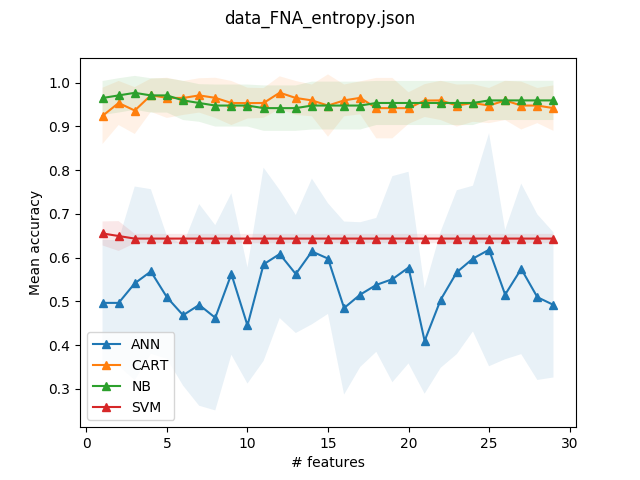
\includegraphics[width=\textwidth]{../plots_with_std_fill/data_FNA_entropy_combined.png}
      \caption[]%
      {{\small}}
      \label{fig:WBCD_entropy}
  \end{subfigure}
  \vskip\baselineskip
  \begin{subfigure}[b]{0.475\textwidth}
      \centering
      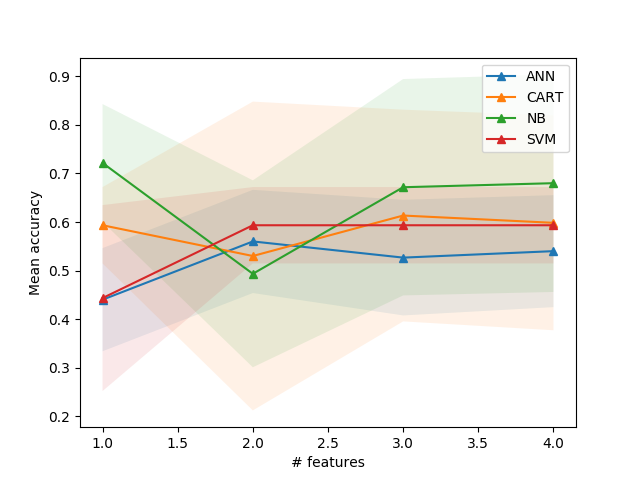
\includegraphics[width=\textwidth]{../plots_with_std_fill/Data_mias_entropy_combined.png}
      \caption[]%
      {{\small }}
      \label{fig:MIAS_entropy}
  \end{subfigure}
  \quad
  \begin{subfigure}[b]{0.475\textwidth}
      \centering
      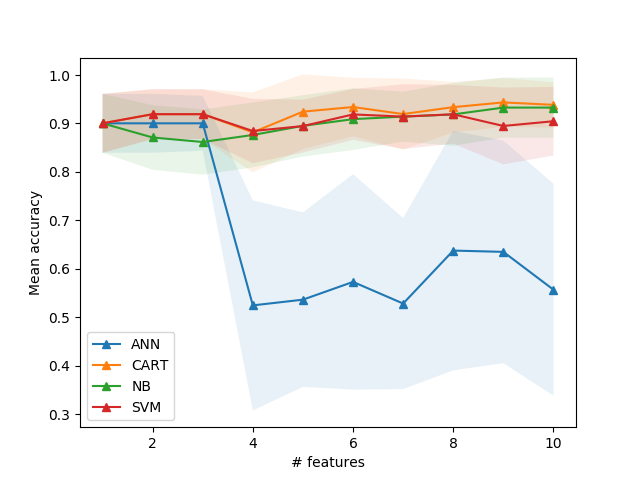
\includegraphics[width=\textwidth]{../plots_with_std_fill/FNA_gb_entropy_combined.png}
      \caption[]%
      {{\small }}
      \label{fig:RHH_entropy}
  \end{subfigure}
  \caption[]
  {{\small a: Dataset EN using Entropy, b: Dataset WBCD using Entropy, c: Dataset MIAS using Entropy, d: Dataset RHH using Entropy. Combined plots of all datasets comparing each classifier when using Entropy for feature selection.}}
  \label{fig:plots_entropy}
\end{figure*}


\subsubsection{Decision Tree}

The decision tree shows consistent performance generally increasing performance with an increased amount of features. Although in cases like plot \ref{fig:WBCD_chi2} and \ref{fig:MIAS_sbs} best accuracy is achieved with a subset of features displaying evident benefits of feature selection.

\begin{figure*}[htp]
  \centering
  \begin{subfigure}[b]{0.475\textwidth}
      \centering
      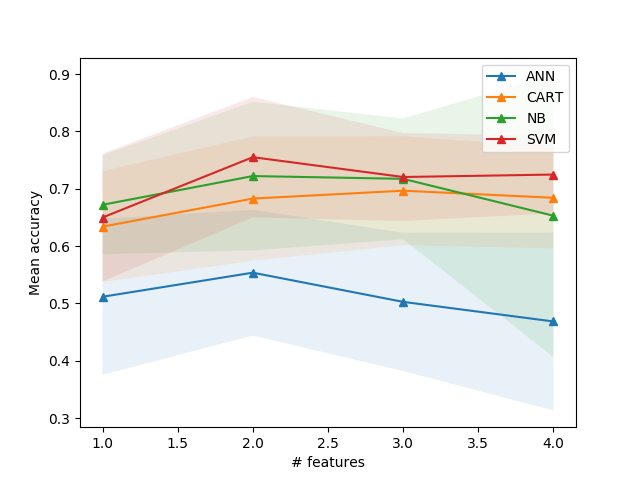
\includegraphics[width=\textwidth]{../plots_with_std_fill/Cleaned_data_sb_combined.png}
      \caption[]%
      {{\small}}
      \label{fig:EN_sbs}
  \end{subfigure}
  \hfill
  \begin{subfigure}[b]{0.475\textwidth}
      \centering
      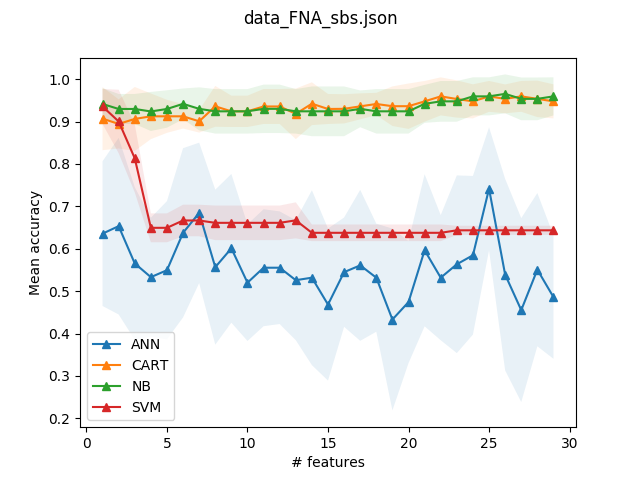
\includegraphics[width=\textwidth]{../plots_with_std_fill/data_FNA_sb_combined.png}
      \caption[]%
      {{\small}}
      \label{fig:WBCD_sbs}
  \end{subfigure}
  \vskip\baselineskip
  \begin{subfigure}[b]{0.475\textwidth}
      \centering
      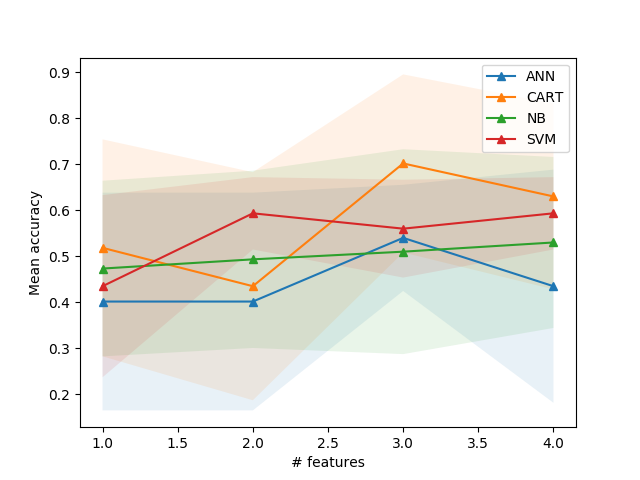
\includegraphics[width=\textwidth]{../plots_with_std_fill/Data_mias_sb_combined.png}
      \caption[]%
      {{\small}}
      \label{fig:MIAS_sbs}
  \end{subfigure}
  \quad
  \begin{subfigure}[b]{0.475\textwidth}
      \centering
      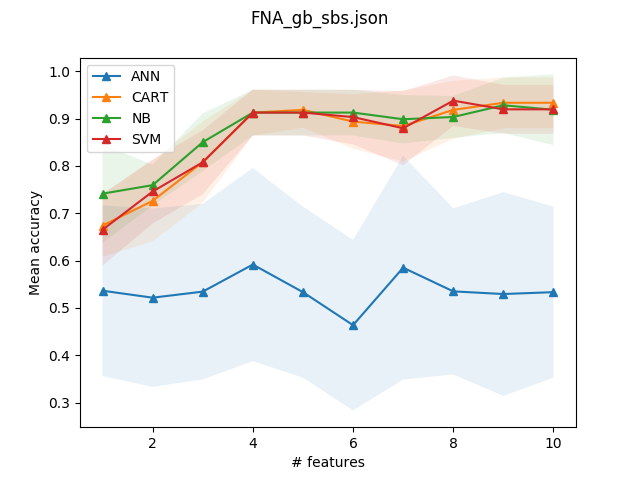
\includegraphics[width=\textwidth]{../plots_with_std_fill/FNA_gb_sb_combined.png}
      \caption[]%
      {{\small}}
      \label{fig:RHH_sbs}
  \end{subfigure}
  \caption[]
  {{\small (a) Dataset EN using SBS. (b) Dataset WBCD using SBS. (c) Dataset MIAS using SBS. (d) Dataset RHH using SBS. Combined plots of all datasets comparing each classifier when using SBS for feature selection.}}
  \label{fig:plots_sbs}
\end{figure*}


\subsubsection{Naive Bayes}

Naive Bayes had the least accumulated gain from feature selection as seen in table \ref{table:gain_comparison}. The largest improvement was seen in plot \ref{fig:EN_chi2} using 2 of 4 available attributes. In plots \ref{fig:WBCD_entropy} and \ref{fig:RHH_entropy} the accuracy sees little to no improvement when increasing the number of attributes.

\begin{figure*}[htbp!]
  \centering
  \begin{subfigure}[b]{0.475\textwidth}
      \centering
      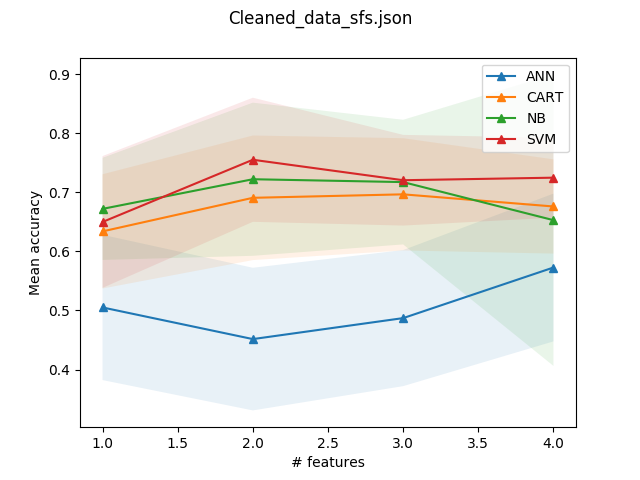
\includegraphics[width=\textwidth]{../plots_with_std_fill/Cleaned_data_sf_combined.png}
      \caption[]%
      {{\small Dataset EN using SFS}}
      \label{fig:EN_sfs}
  \end{subfigure}
  \hfill
  \begin{subfigure}[b]{0.475\textwidth}
      \centering
      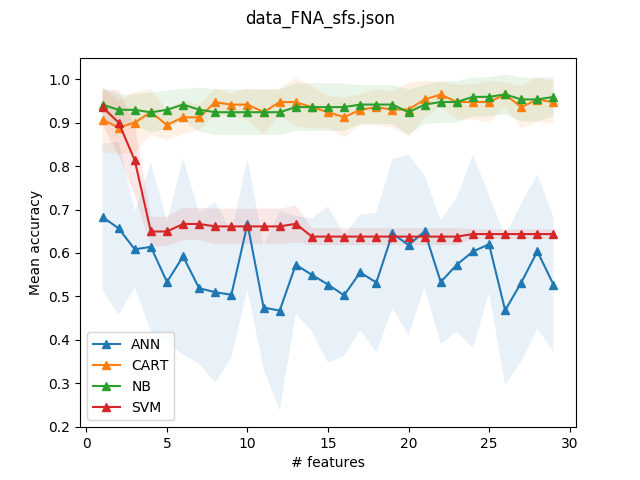
\includegraphics[width=\textwidth]{../plots_with_std_fill/data_FNA_sf_combined.png}
      \caption[]%
      {{\small Dataset WBCD using SFS}}
      \label{fig:WBCD_sfs}
  \end{subfigure}
  \vskip\baselineskip
  \begin{subfigure}[b]{0.475\textwidth}
      \centering
      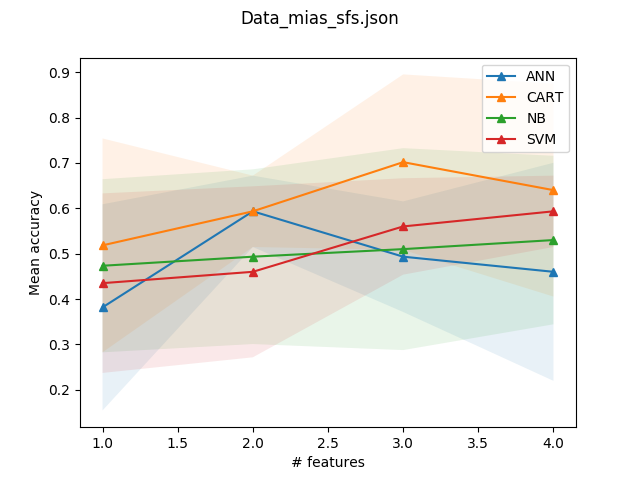
\includegraphics[width=\textwidth]{../plots_with_std_fill/Data_mias_sf_combined.png}
      \caption[]%
      {{\small Dataset MIAS using SFS}}
      \label{fig:MIAS_sfs}
  \end{subfigure}
  \quad
  \begin{subfigure}[b]{0.475\textwidth}
      \centering
      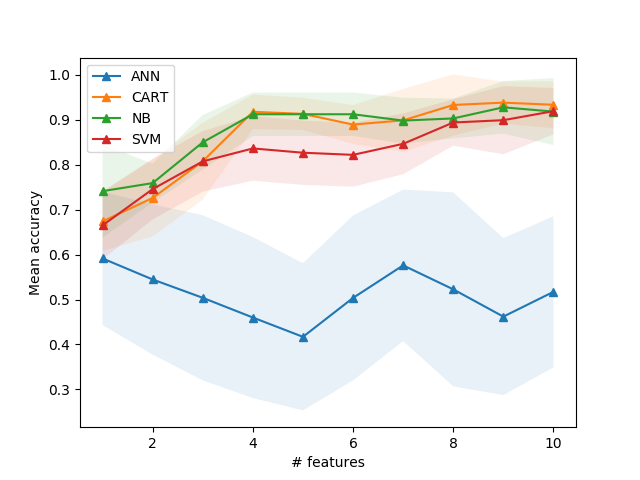
\includegraphics[width=\textwidth]{../plots_with_std_fill/FNA_gb_sf_combined.png}
      \caption[]%
      {{\small Dataset RHH using SFS}}
      \label{fig:RHH_sfs}
  \end{subfigure}
  \caption[]
  {{\small Combined plots of all datasets comparing each classifier when using SFS for feature selection.}}
  \label{fig:plots_sfs}
\end{figure*}



\section{Computation time}

\textbf{Under construction, profiling not run yet.}

Profiling the execution of running all experiments X\% of CPU-time was allocated to the Wrapper algorithms. As mentioned a finding the best possible subset of features is considered a NP-hard problem meaning a solution can not be found in polynomial time. This clearly suggest favouring filtering methods when choosing a feature selection method having limited computational resources.

\section{Source of errors}
\label{sec:source_of_errors}

There are two main factor that may risk propagate error into the results, libraries and datasets.

The libraries provide all functionality of the classifiers and the filter selection methods, thus a major part of the implementation. A implementation built upon faulty methods can not provide any significant results. We use two libraries. The Scikit library \parencite{scikit-learn} is well renowned widely used in both industry and research thus inspire confidence in its robustness. The mlxtend library is used for SBS and SFS methods and is still a open source with less coverage than Scikit \parencite{mlextend}. Still it has a active community and many release versions indicating it's well managed.

Datasets... \textbf{Under construction...}

% Source of error can be expanded here, discuss effect of binary classification and chance of subsets containing only one class. This is addressed with stratifiedKfold but in data poor sets the problem can still remain
